\documentclass[]{elsarticle} %review=doublespace preprint=single 5p=2 column
%%% Begin My package additions %%%%%%%%%%%%%%%%%%%
\usepackage[hyphens]{url}

  \journal{PH 682} % Sets Journal name


\usepackage{lineno} % add
\providecommand{\tightlist}{%
  \setlength{\itemsep}{0pt}\setlength{\parskip}{0pt}}

\usepackage{graphicx}
%%%%%%%%%%%%%%%% end my additions to header

\usepackage[T1]{fontenc}
\usepackage{lmodern}
\usepackage{amssymb,amsmath}
\usepackage{ifxetex,ifluatex}
\usepackage{fixltx2e} % provides \textsubscript
% use upquote if available, for straight quotes in verbatim environments
\IfFileExists{upquote.sty}{\usepackage{upquote}}{}
\ifnum 0\ifxetex 1\fi\ifluatex 1\fi=0 % if pdftex
  \usepackage[utf8]{inputenc}
\else % if luatex or xelatex
  \usepackage{fontspec}
  \ifxetex
    \usepackage{xltxtra,xunicode}
  \fi
  \defaultfontfeatures{Mapping=tex-text,Scale=MatchLowercase}
  \newcommand{\euro}{€}
\fi
% use microtype if available
\IfFileExists{microtype.sty}{\usepackage{microtype}}{}
\bibliographystyle{elsarticle-harv}
\usepackage{graphicx}
\ifxetex
  \usepackage[setpagesize=false, % page size defined by xetex
              unicode=false, % unicode breaks when used with xetex
              xetex]{hyperref}
\else
  \usepackage[unicode=true]{hyperref}
\fi
\hypersetup{breaklinks=true,
            bookmarks=true,
            pdfauthor={},
            pdftitle={San Diego County Access to Healthy Foods and Prevalence of High Blood Cholesterol, A Cross-sectional Examination of 2019},
            colorlinks=true,
            urlcolor=blue,
            linkcolor=magenta,
            pdfborder={0 0 0}}
\urlstyle{same}  % don't use monospace font for urls

\setcounter{secnumdepth}{0}
% Pandoc toggle for numbering sections (defaults to be off)
\setcounter{secnumdepth}{0}

% Pandoc citation processing
\newlength{\cslhangindent}
\setlength{\cslhangindent}{1.5em}
\newlength{\csllabelwidth}
\setlength{\csllabelwidth}{3em}
% for Pandoc 2.8 to 2.10.1
\newenvironment{cslreferences}%
  {}%
  {\par}
% For Pandoc 2.11+
\newenvironment{CSLReferences}[2] % #1 hanging-ident, #2 entry spacing
 {% don't indent paragraphs
  \setlength{\parindent}{0pt}
  % turn on hanging indent if param 1 is 1
  \ifodd #1 \everypar{\setlength{\hangindent}{\cslhangindent}}\ignorespaces\fi
  % set entry spacing
  \ifnum #2 > 0
  \setlength{\parskip}{#2\baselineskip}
  \fi
 }%
 {}
\usepackage{calc}
\newcommand{\CSLBlock}[1]{#1\hfill\break}
\newcommand{\CSLLeftMargin}[1]{\parbox[t]{\csllabelwidth}{#1}}
\newcommand{\CSLRightInline}[1]{\parbox[t]{\linewidth - \csllabelwidth}{#1}\break}
\newcommand{\CSLIndent}[1]{\hspace{\cslhangindent}#1}

% Pandoc header
\usepackage{setspace}\doublespacing \usepackage{floatrow} \floatsetup[figure]{capposition=top} \floatsetup[table]{capposition=top}
\usepackage{booktabs}
\usepackage{longtable}
\usepackage{array}
\usepackage{multirow}
\usepackage{wrapfig}
\usepackage{float}
\usepackage{colortbl}
\usepackage{pdflscape}
\usepackage{tabu}
\usepackage{threeparttable}
\usepackage{threeparttablex}
\usepackage[normalem]{ulem}
\usepackage{makecell}
\usepackage{xcolor}



\begin{document}
\begin{frontmatter}

  \title{San Diego County Access to Healthy Foods and Prevalence of High
Blood Cholesterol, A Cross-sectional Examination of 2019}
    \author[San Diego State University School of Public
Health]{Christian Hicks}
   \ead{chicks5799@sdsu.edu} 
      
  \begin{abstract}
  \textbf{Background:} High cholesterol is a risk factor for heart
  disease and mortality. Poor diet can lead to the development of high
  cholesterol, therefore it is important to study individuals' access to
  healthy foods. \textbf{Methods:} High cholesterol prevalences and
  grocery store locations were examined in San Diego County Census
  tracts to determine the distributions and if the two are associated.
  Data was obtained from sources provided by the CDC and Esri.
  \textbf{Results:} It was observed that a moderate negative association
  was present between high cholesterol prevalence and number of nearby
  grocery stores (R = -0.32, p\textless.001). \textbf{Conclusion:} These
  results suggest that access to grocery stores may affect the health
  status of San Diego County residents.
  \end{abstract}
  
 \end{frontmatter}

\hypertarget{introduction}{%
\section{Introduction}\label{introduction}}

\hypertarget{background}{%
\paragraph{Background}\label{background}}

Heart disease was the leading cause of death in San Diego County between
1999 and 2019 with a crude rate of 210 deaths per 100,000 adults
(\protect\hyperlink{ref-wonder2019}{CDC, 2020}). Diabetes was ranked as
the seventh leading cause of death in this region and time period with a
crude rate of 25 deaths per 100,000 adults
(\protect\hyperlink{ref-wonder2019}{CDC, 2020}). Recent studies have
focused on examining features of U.S. neighborhood structures and how it
may affect individual health
(\protect\hyperlink{ref-havranek2015}{Havranek et al., 2015};
\protect\hyperlink{ref-morris19}{Morris et al., 19 C.E.}). Specifically
the Multi-Ethnic Study of Atherosclerosis (MESA), a longitudinal study
of cardiovascular disease, linked access to healthy food with reduced
risk factors of morbidity
(\protect\hyperlink{ref-auchincloss2013}{Auchincloss et al., 2013}).

\hypertarget{purpose}{%
\paragraph{Purpose}\label{purpose}}

San Diego County has many urban, suburban, and rural neighborhoods with
various levels of access to grocery stores. This study explored how the
count and location of grocery stores related to prevalence of high
cholesterol within census tracts. Cross-sectional data of high
cholesterol prevalence were compared with business location data in San
Diego County. It was hypothesized that increased access to grocery
stores would be associated with lower prevalence of high cholesterol.

\hypertarget{methods}{%
\section{Methods}\label{methods}}

\hypertarget{data-collection}{%
\paragraph{Data collection}\label{data-collection}}

High cholesterol prevalence data was provided by the CDC PLACES project
(\protect\hyperlink{ref-cdc2021}{CDC, 2021}). Data used from this source
was limited to San Diego County and its 626 Census tracts' boundaries.
One Census tract out of the 626 was removed from analysis due to it
consisting entirely of a U.S. Marine base. The CDC PLACES population
data estimates are derived from the CDC Behavior Risk Factor
Surveillance System, the Census 2010 population, the American Community
Survey, and other nationwide health surveys.

Community access to healthy foods was determined using grocery store
location data from the ArcGIS Community Analyst online service
(\protect\hyperlink{ref-esri2021}{Esri, n.d.}). The Business and
Facilities Search tool from this service was used to obtain necessary
information on all businesses in San Diego County labelled as a grocery
retail store. The data obtained from this source was provided by Data
Axle company (\protect\hyperlink{ref-dataaxle2021}{Data-Axle, n.d.}).

\hypertarget{statistical-analyses}{%
\paragraph{Statistical Analyses}\label{statistical-analyses}}

ArcGIS Pro 2.8.3 was used for all spatial analyses and R 4.1.1 was used
for statistical analyses. Trends and abnormalities in the distribution
of high cholesterol prevalence was determined by comparing Census tracts
with each other. Grocery store density within San Diego County was
calculated using the Kernel Density tool from ArcGIS Pro. This tool is
based on a formula described on page 76 in the book \emph{Density
Estimation for Statistics and Data Analysis}
(\protect\hyperlink{ref-silverman1986}{Silverman, 1986}). Census tracts
were joined with grocery store locations to count the number of grocery
stores within the boundaries of each Census tract in addition to grocery
stores within a mile of those boundaries.

To numerically describe the relationship between prevalence points and
number of nearby grocery stores within each Census tract, high
cholesterol prevalence was normalized on a per grocery store basis. This
was used to describe how many prevalence points existed alongside an
average grocery store. Examination of the relationship between these two
variables was performed by using generalized linear regression to
predict Census tract high cholesterol prevalence using the number of
nearby grocery stores. Residuals of this model were mapped to identify
outlying over- and underestimations of high cholesterol prevalence.

\hypertarget{results}{%
\section{Results}\label{results}}

\hypertarget{descriptive-statistics}{%
\paragraph{Descriptive Statistics}\label{descriptive-statistics}}

The median high cholesterol prevalence was 28.5\% (8.8 - 45.0\%).
Distribution of high cholesterol prevalence throughout San Diego County
is shown in \textbf{Figure \ref{fig1}}. The median number of nearby
grocery stores was 10 (0 - 52). There were eight Census tracts that did
not have a grocery store either within their boundaries or within a mile
of their boundaries. The median prevalence of high cholesterol with
these eight tracts was 33.0\% (30.0 - 36.8\%)

\begin{table}

\caption{\label{tab:tableone_print}Demographics}
\centering
\begin{tabular}[t]{ll}
\toprule
  & Value\\
\midrule
Census tracts (n) & 625\\
High cholesterol prevalence (\%) & 28.54 (4.19)\\
Nearby grocery stores & 10.00 [0.00, 52.00]\\
Total population & 4630.00 [144.00, 28960.00]\\
Census tract square mileage & 0.78 [0.10, 1068.16]\\
\bottomrule
\multicolumn{2}{l}{\rule{0pt}{1em}\textit{Note: }}\\
\multicolumn{2}{l}{\rule{0pt}{1em}mean (SD); median [min, max]}\\
\end{tabular}
\end{table}

\hypertarget{grocery-store-density}{%
\paragraph{Grocery Store Density}\label{grocery-store-density}}

Density of grocery stores throughout San Diego County was rasterized in
\textbf{Figure \ref{fig2}}. The downtown metropolitan region of San
Diego County had the greatest density of grocery stores. In the northern
region, the greatest density was observed along the California SR-78
highway from Oceanside to Escondido. Number of grocery stores within a
Census tract and within a mile of a tract's boundaries were shown with
\textbf{Figure \ref{fig3}}. The downtown tracts with the greatest number
of nearby grocery stores were within the neighborhoods of East Village,
Logan Heights, South Park, and North Park. Areas around the San Diego
State University also had large numbers of nearby grocery stores,
specifically the neighborhoods of College West and City Heights.

\hypertarget{relationship-between-high-cholesterol-and-nearby-grocery-stores}{%
\paragraph{Relationship Between High Cholesterol and Nearby Grocery
Stores}\label{relationship-between-high-cholesterol-and-nearby-grocery-stores}}

High cholesterol prevalence points per grocery store were mapped by San
Diego County Census tracts in \textbf{Figure \ref{fig4}}. The median
high cholesterol prevalence points per grocery store was 3.0\% (0.5 -
39.9\%). Over 90\% of tracts had 10 prevalence points or fewer for every
nearby grocery store.

\hypertarget{generalized-linear-regression-and-residuals}{%
\paragraph{Generalized Linear Regression and
Residuals}\label{generalized-linear-regression-and-residuals}}

There is a moderate negative correlation between high cholesterol
prevalence and nearby grocery stores (R = -0.32, p\textless.001). When
fit to a linear regression model, every 10 nearby grocery stores was
associated with a decrease in the average Census tract's high
cholesterol prevalence by 1.6\% (95\% CI = -2.0\%, -1.2\%). Each Census
tract's residual from this model was shown in \textbf{Figure
\ref{fig5}}. Three tracts in the northern half of San Diego County had
their residuals greater than 2.5 standard deviations from the predicted
high cholesterol prevalence. Fifteen tracts in the south western region
had residuals less than -2.5 standard deviations from the the predicted
prevalence.

\hypertarget{discussion}{%
\section{Discussion}\label{discussion}}

The moderate negative correlation between high cholesterol prevalence
and number of nearby grocery stores may suggest that access to healthy
foods may affect individual health in the county of San Diego. Many of
the Census tracts with large high cholesterol prevalences and few
grocery store options were located away from the urbanized areas of the
county. For example, nearly all of the rural Census tracts had a high
cholesterol prevalence greater than the mean. This could likely be due
to the distance of the nearest grocery store and lack of variety to
choose from. Tracts within the densely populated urban areas often had
high counts of nearby grocery stores and relatively low prevalences of
high cholesterol.

Variables included in the regression models were limited to those
provided by the data sources used in this research. Collection and use
of more variables such as individual demographic characteristics may
allow for the development of a stronger model. Another method to improve
accuracy of analyses would be to include street and sidewalk data to
determine the travel distance to grocery stores rather than the general
spatial distance. This would be more realistic as it could estimate the
time required of an individual to travel to grocery store locations.

The residual outliers displayed in \textbf{Figure \ref{fig5}} represent
Census tracts that either had large high cholesterol prevalences
regardless of the many grocery store options, or low prevalences with
little or no nearby grocery stores. A possible explanation could be the
presence of parks and various outdoor activities, or a lack thereof.
Further research into these Census tracts is needed to determine
potential factors in this observed finding.

\hypertarget{conclusion}{%
\section{Conclusion}\label{conclusion}}

High cholesterol is a risk factor of heart disease, the modern number
one cause of death in San Diego County. The effect of environmental
factors, such as neighborhood structure, upon individual health
continues to be widely researched. This study provides evidence
supporting the hypothesis that a lack of access to healthy foods is
associated with impaired health statuses. Further research is needed to
strengthen this conclusion and provide vital information to public
policy making processes.

\pagebreak

\begin{figure}
\centering
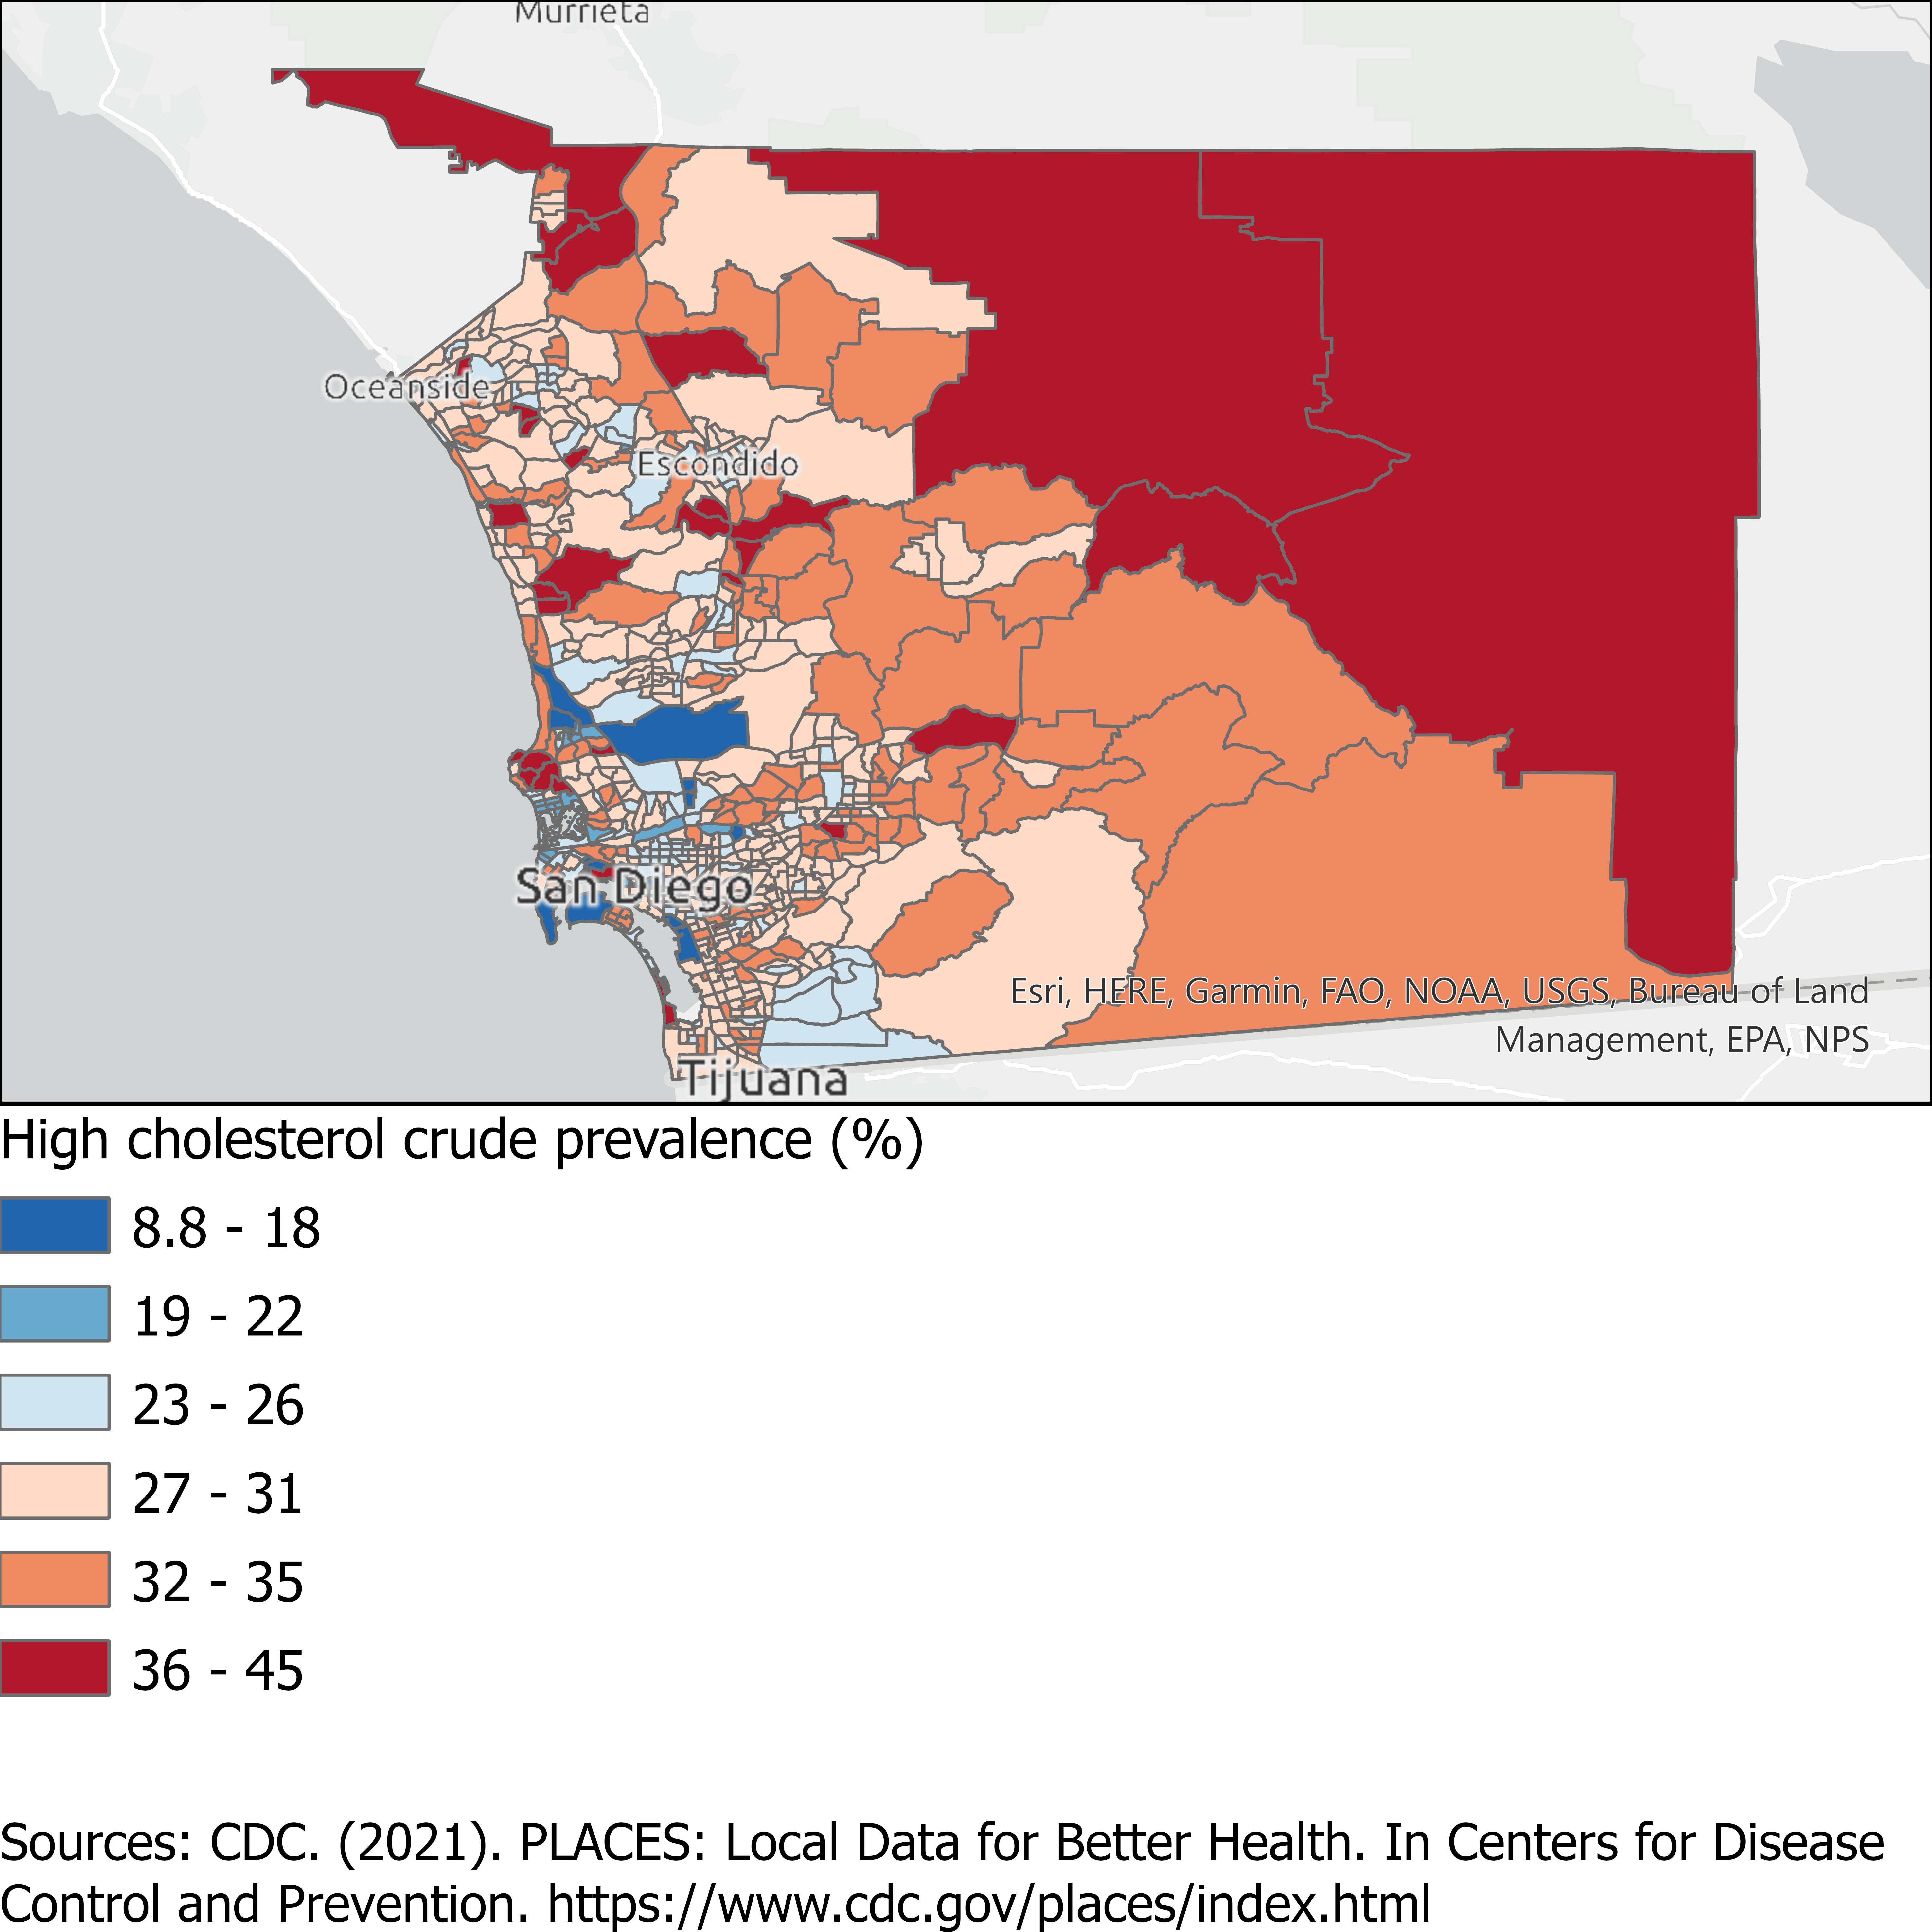
\includegraphics{"../map1.png"}
\caption{High cholesterol prevalence by San Diego County Census
tracts.\label{fig1}}
\end{figure}

\begin{figure}
\centering
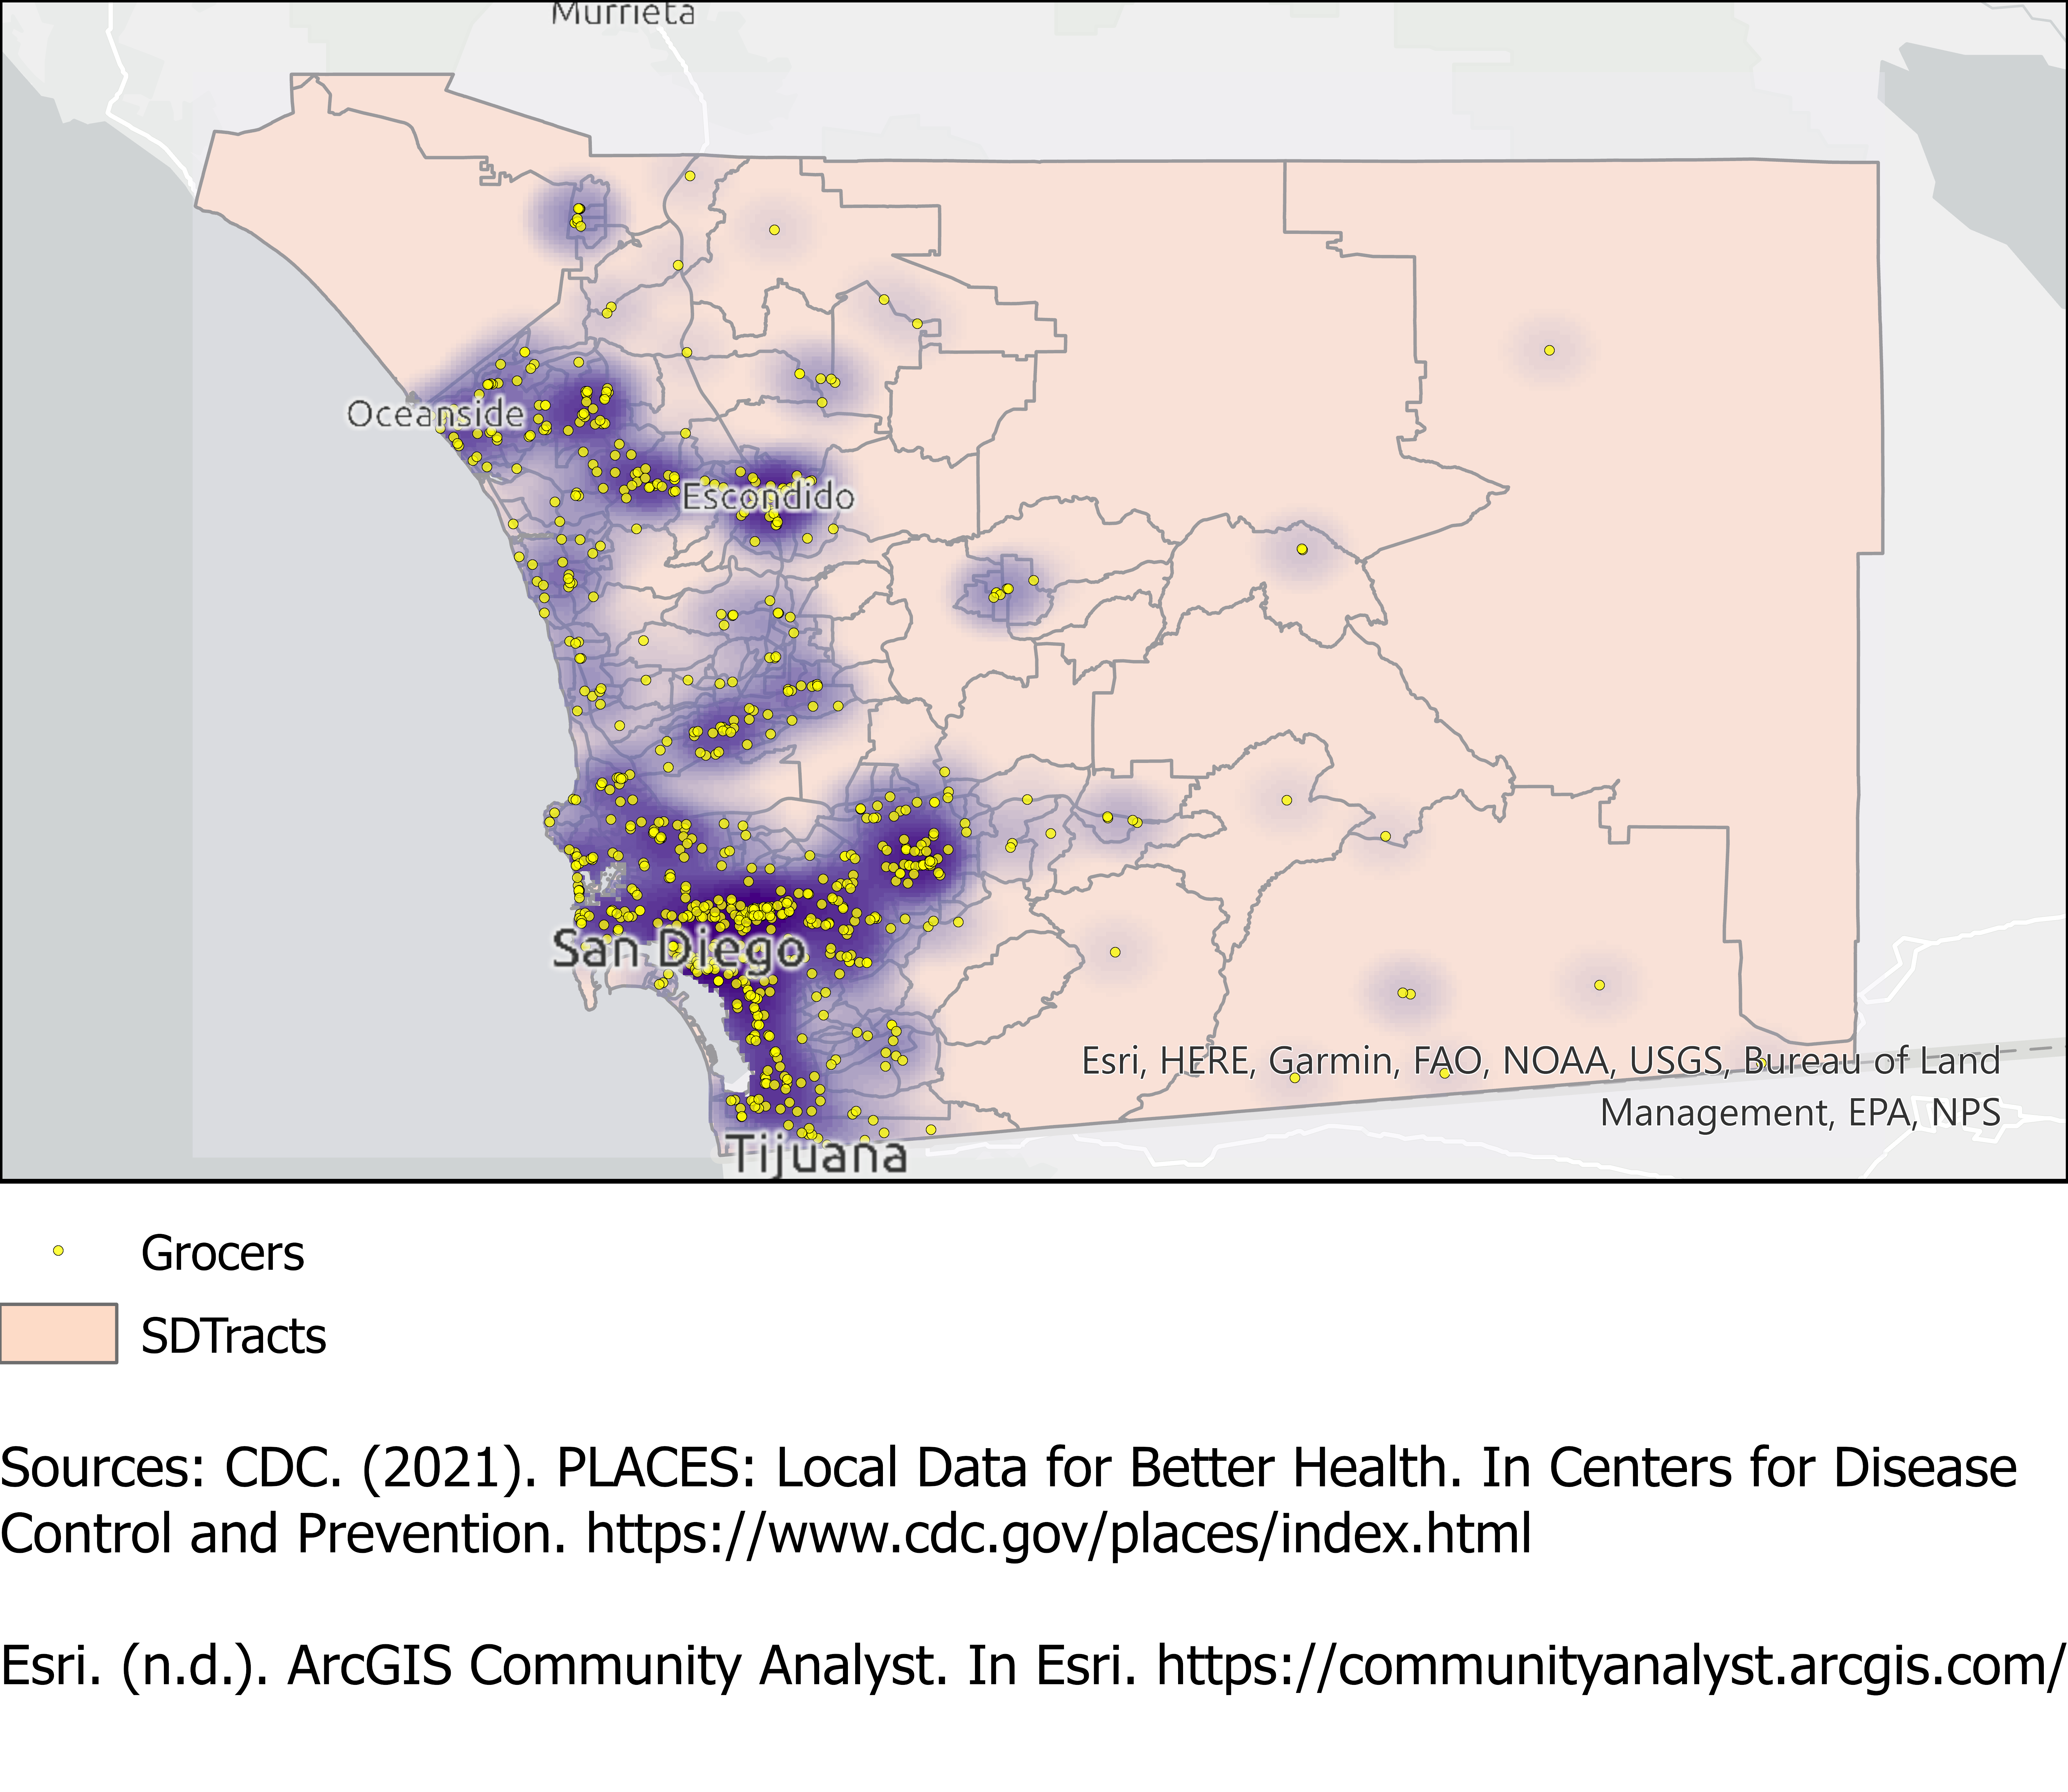
\includegraphics{"../map2.png"}
\caption{Grocery store density throughout San Diego County.\label{fig2}}
\end{figure}

\begin{figure}
\centering
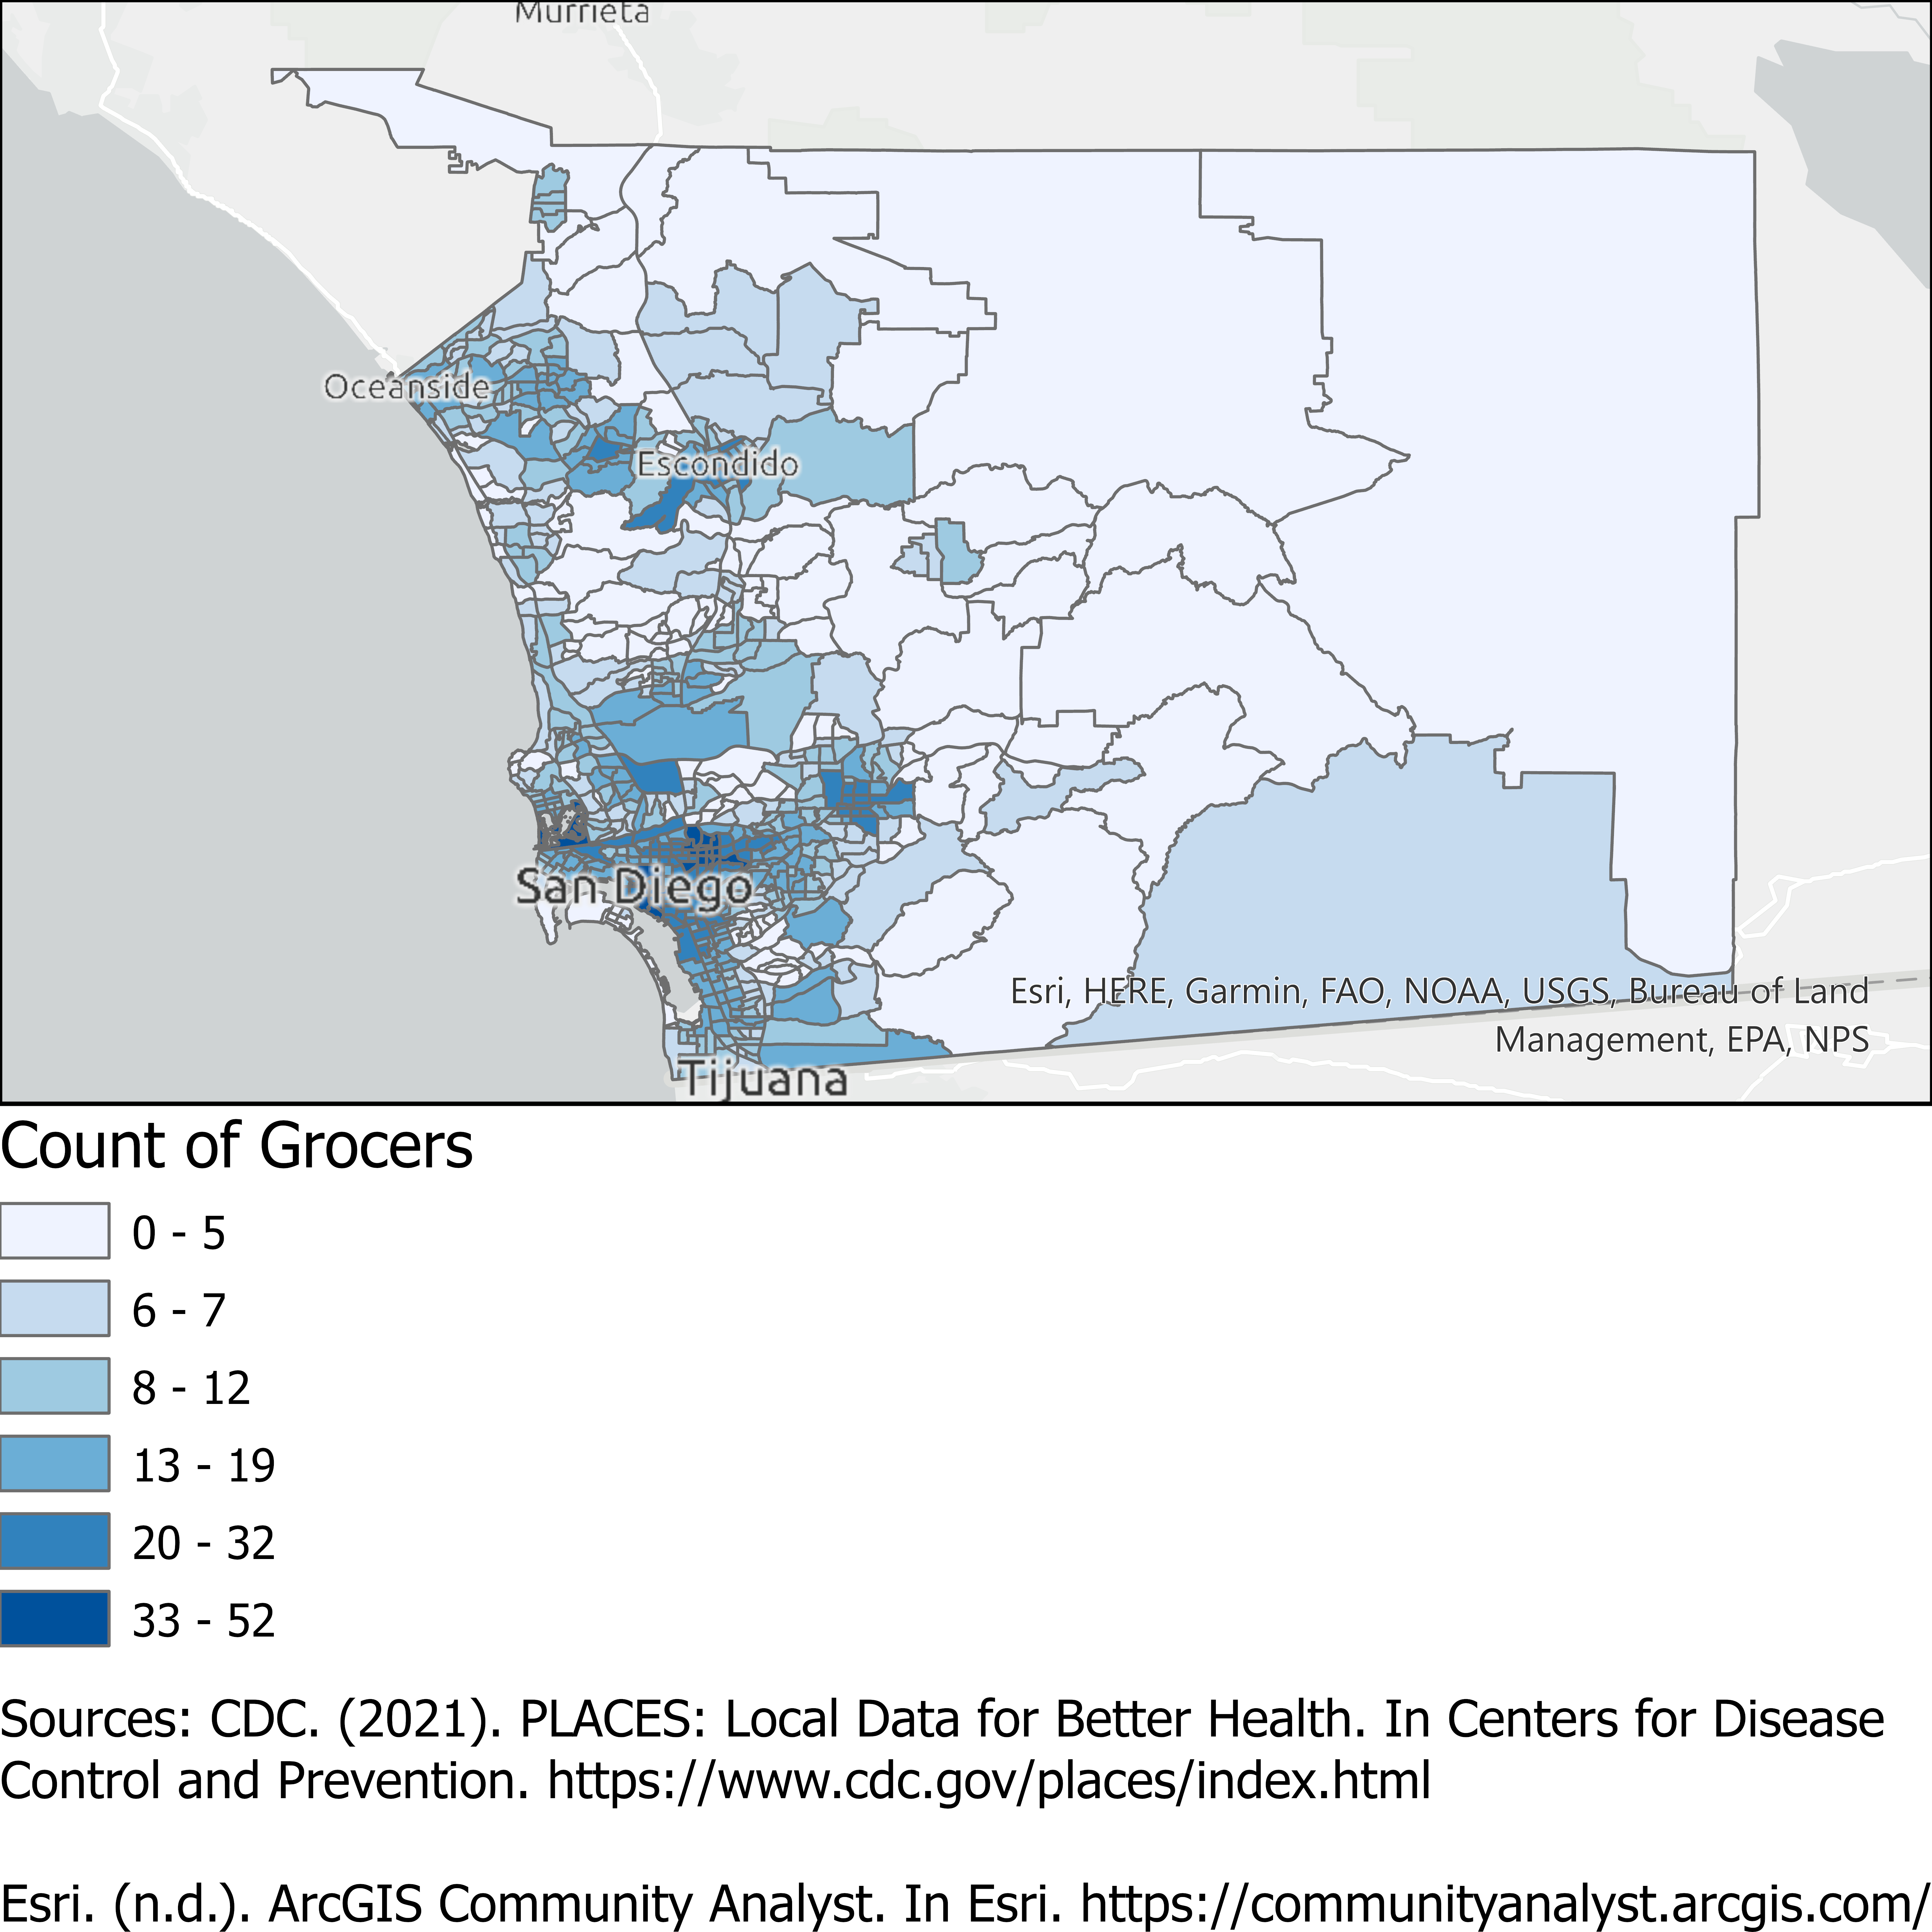
\includegraphics{"../map3.png"}
\caption{Number of grocery stores inside or within one mile of San Diego
Census tracts.\label{fig3}}
\end{figure}

\begin{figure}
\centering
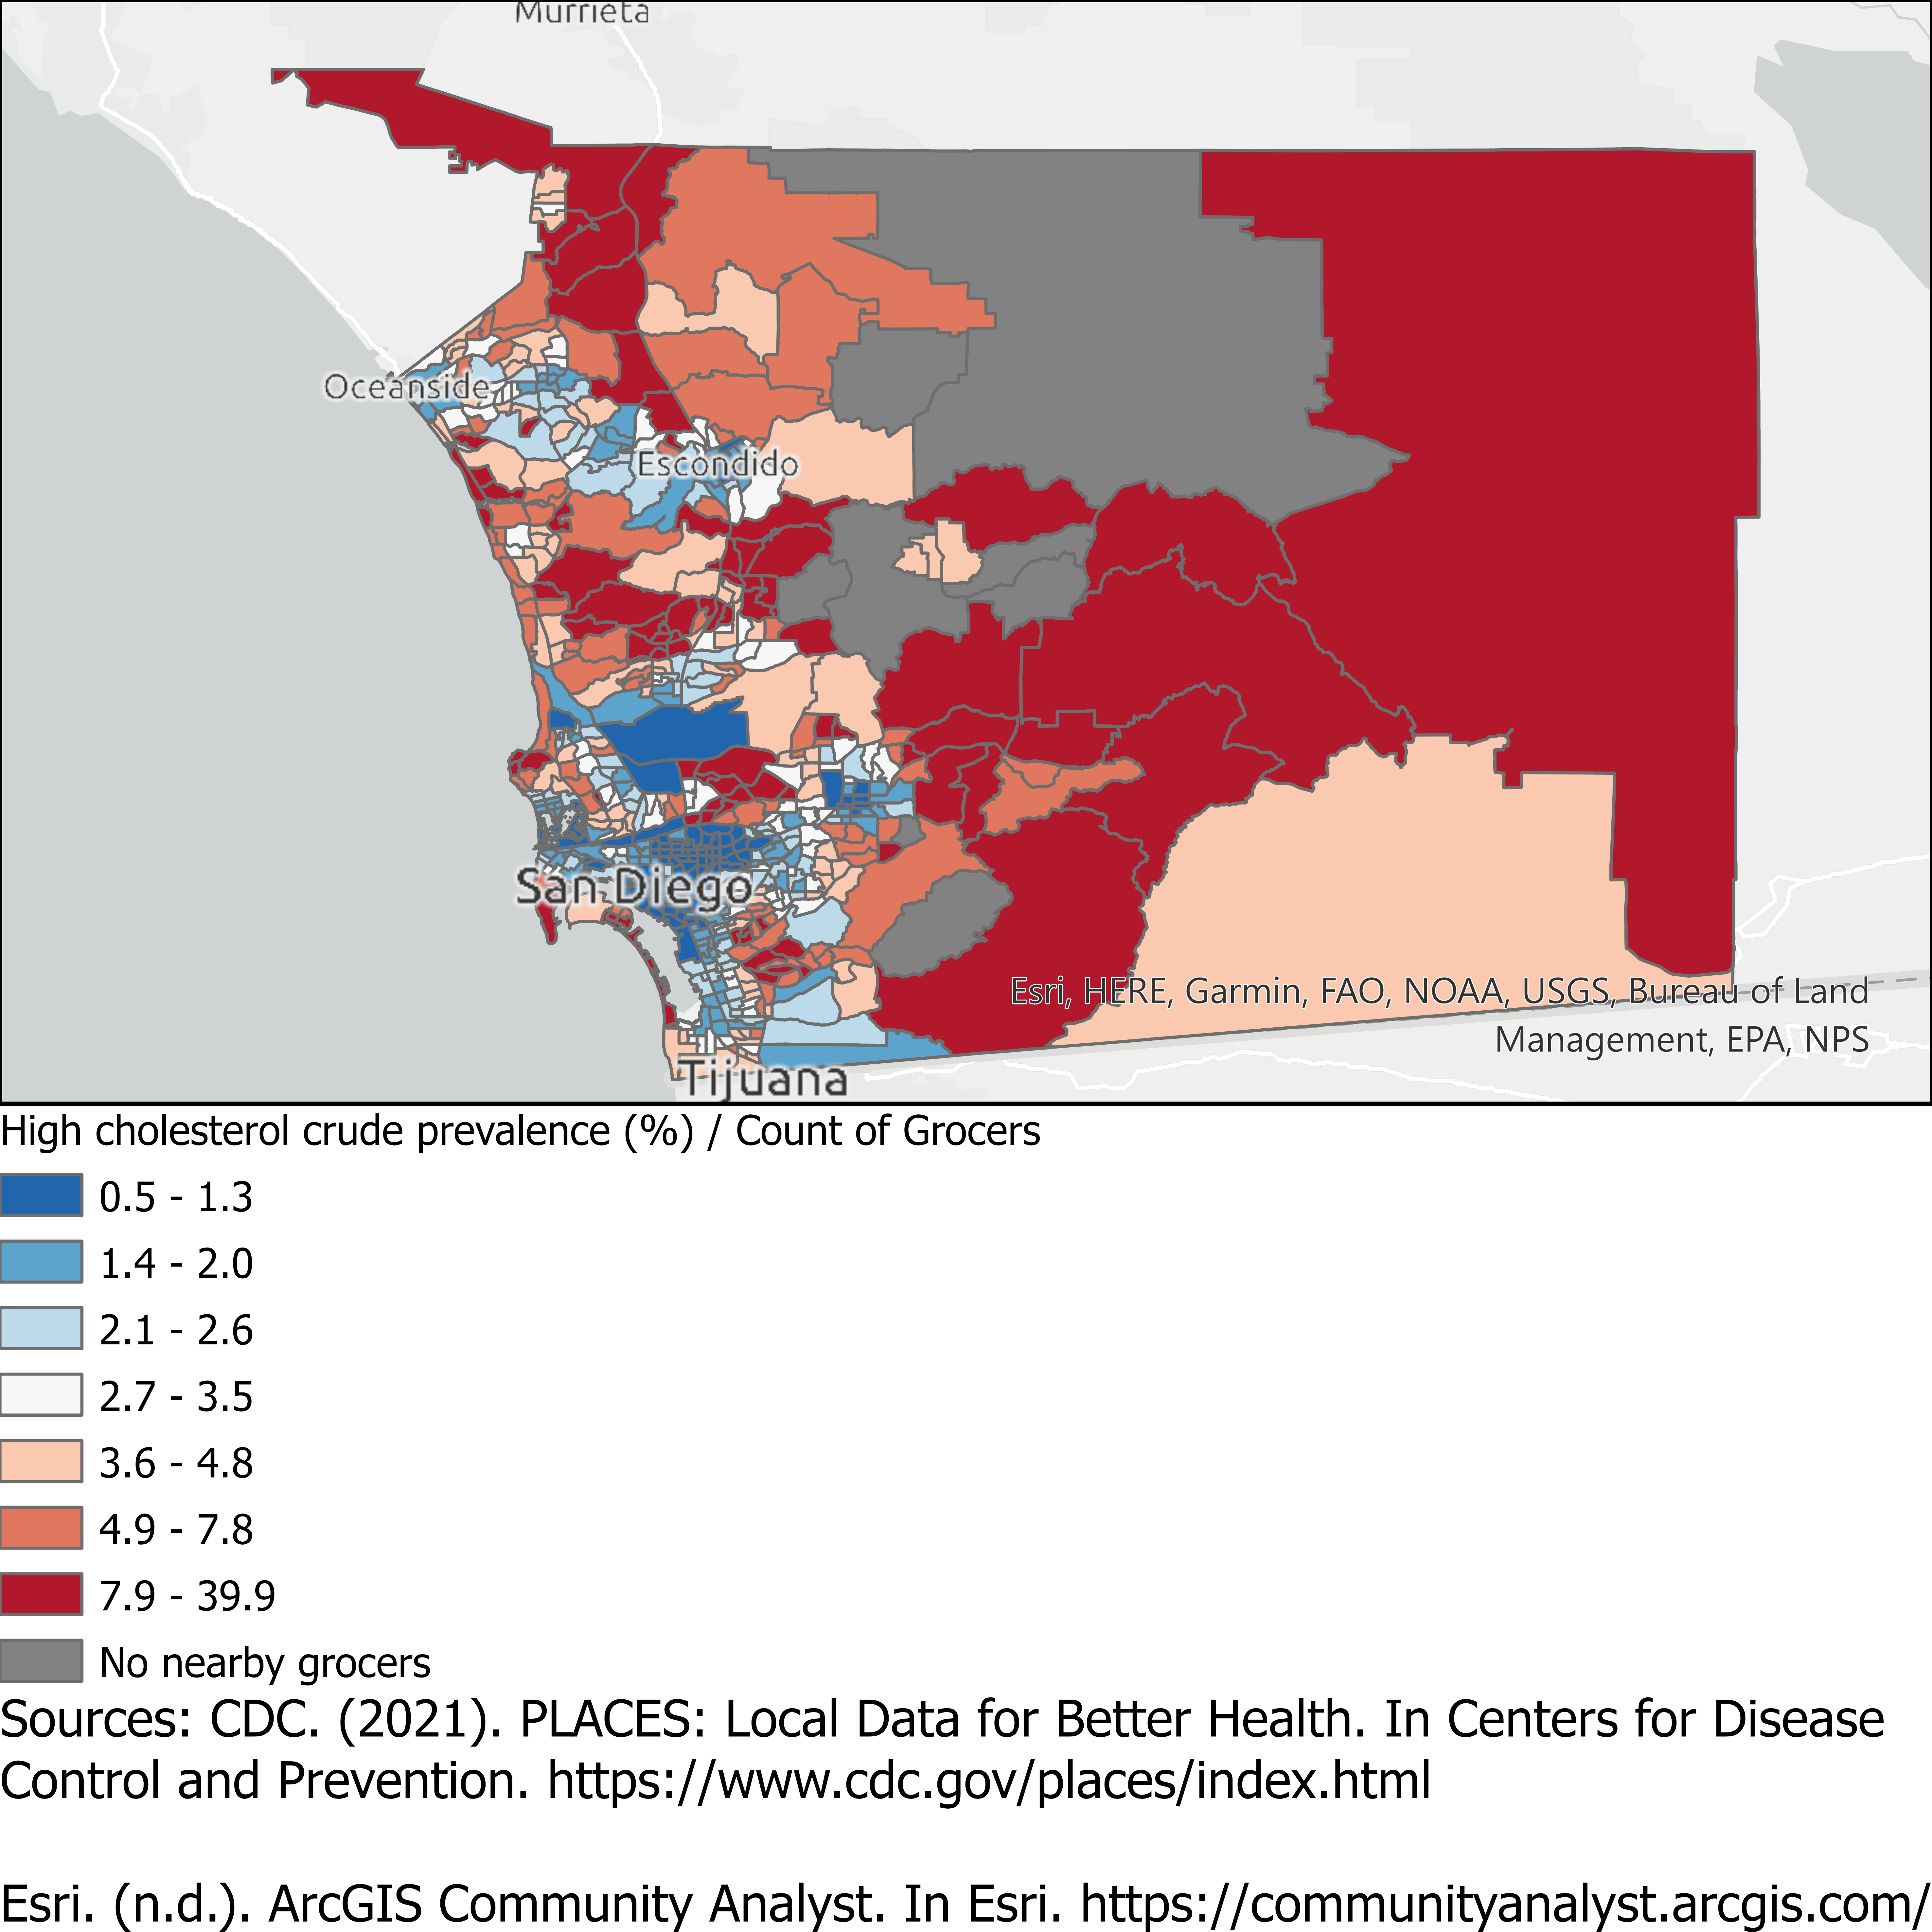
\includegraphics{"../map4.png"}
\caption{High cholesteroal prevalence points per grocery store by San
Diego County Census tracts.\label{fig4}}
\end{figure}

\begin{figure}
\centering
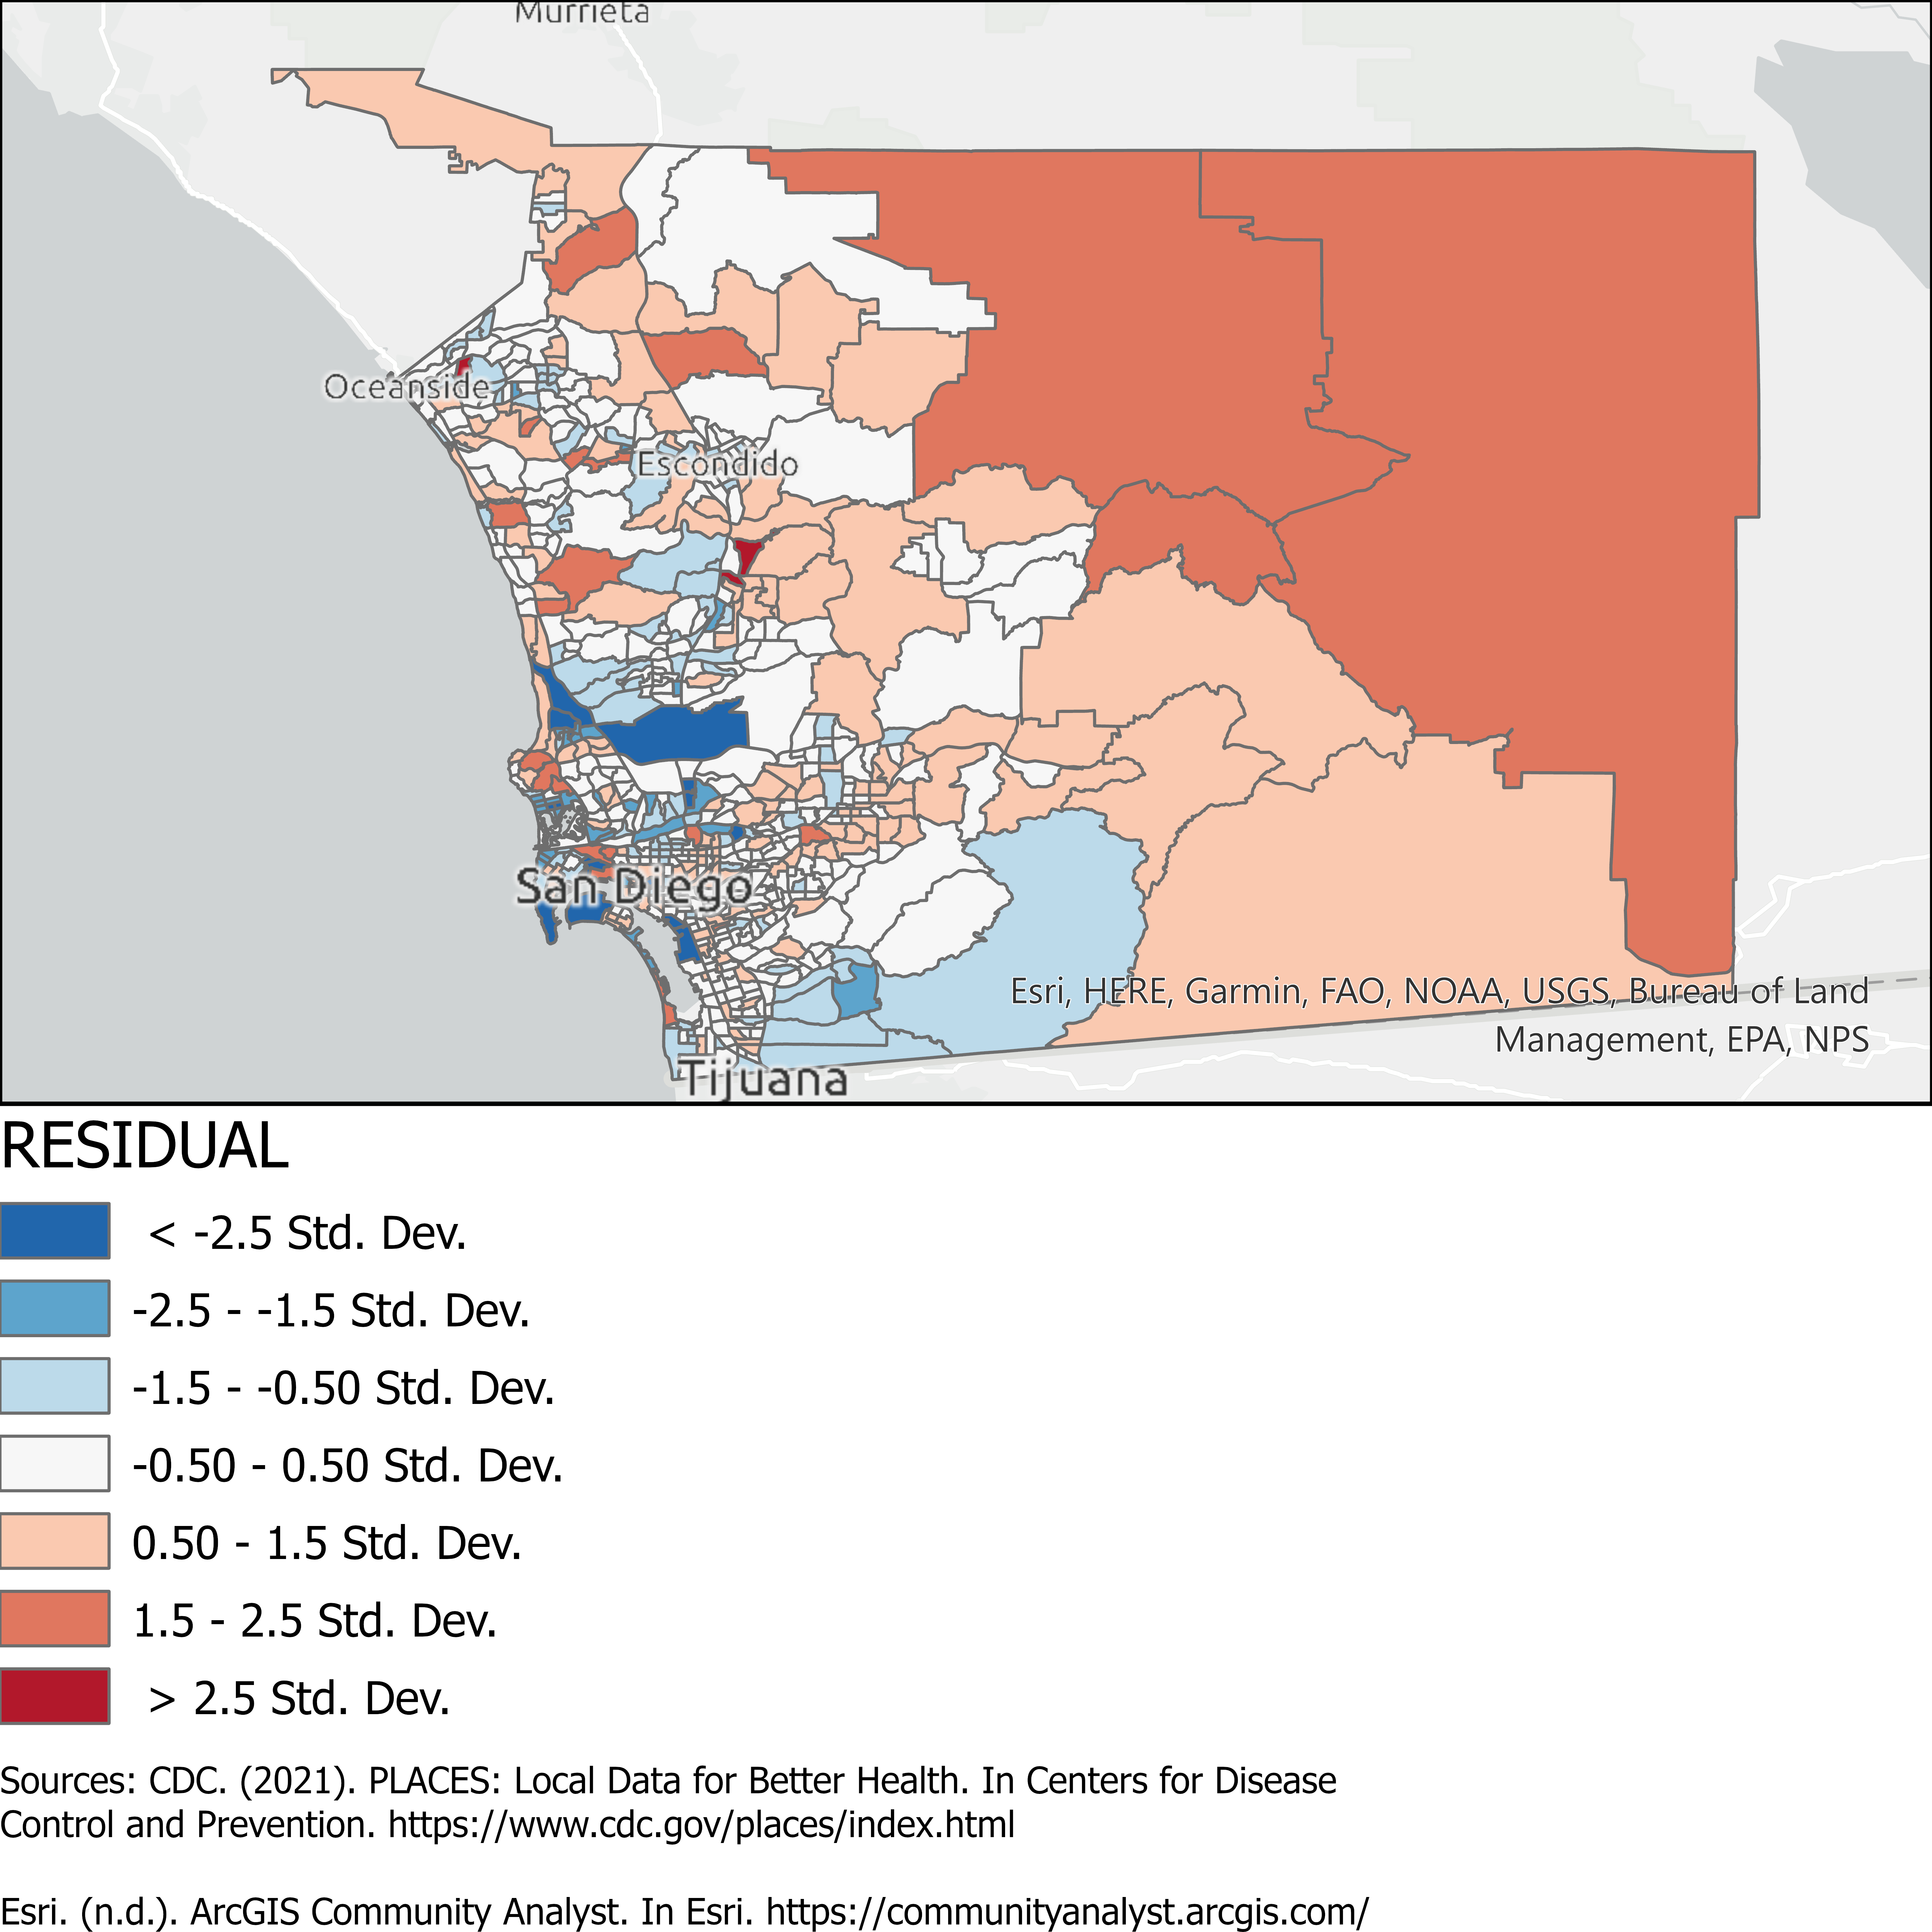
\includegraphics{"../map5.png"}
\caption{Standardized residuals of generalized linear model by San Diego
County Census tracts.\label{fig5}}
\end{figure}

\hypertarget{references}{%
\section*{References}\label{references}}
\addcontentsline{toc}{section}{References}

\hypertarget{refs}{}
\begin{CSLReferences}{1}{0}
\leavevmode\vadjust pre{\hypertarget{ref-auchincloss2013}{}}%
Auchincloss, A. H., Mujahid, M. S., Shen, M., Michos, E. D.,
Whitt-Glover, M. C., \& Diez Roux, A. V. (2013). Neighborhood
health-promoting resources and obesity risk (the multi-ethnic study of
atherosclerosis). \emph{Obesity}, \emph{21}(3), 621--628.
\url{https://doi.org/10.1002/oby.20255}

\leavevmode\vadjust pre{\hypertarget{ref-cdc2021}{}}%
CDC. (2021). {PLACES}: {Local Data} for {Better Health}. In
\emph{Centers for Disease Control and Prevention}.
https://www.cdc.gov/places/index.html.

\leavevmode\vadjust pre{\hypertarget{ref-wonder2019}{}}%
CDC. (2020). Underlying {Cause} of {Death}, 1999-2019 {Results}. In
\emph{CDC WONDER}. http://wonder.cdc.gov/ucd-icd10.html.

\leavevmode\vadjust pre{\hypertarget{ref-dataaxle2021}{}}%
Data-Axle. (n.d.). Data {Axle} - helping businesses make money through
data, technology, \& services. In \emph{Data Axle}.
https://www.data-axle.com/.

\leavevmode\vadjust pre{\hypertarget{ref-esri2021}{}}%
Esri. (n.d.). {ArcGIS Community Analyst}. In \emph{Esri}.
https://communityanalyst.arcgis.com/.

\leavevmode\vadjust pre{\hypertarget{ref-havranek2015}{}}%
Havranek, E. P., Mujahid, M. S., Barr, D. A., Blair, I. V., Cohen, M.
S., Cruz-Flores, S., Davey-Smith, G., Dennison-Himmelfarb, C. R., \&
Lauer, M. S. (2015). Social {Determinants} of {Risk} and {Outcomes} for
{Cardiovascular Disease}: {A Scientific Statement From} the {American
Heart Association}. \emph{Circulation}, \emph{132}(9), 873--898.
\url{https://doi.org/10.1161/CIR.0000000000000228}

\leavevmode\vadjust pre{\hypertarget{ref-morris19}{}}%
Morris, A. A., McAllister, P., Grant, A., Geng, S., Kelli, H. M.,
Kalogeropoulos, A., Quyyumi, A., \& Butler, J. (19 C.E.). Relation of
{Living} in a {``{Food Desert}''} to {Recurrent Hospitalizations} in
{Patients With Heart Failure}. \emph{The American Journal of
Cardiology}, \emph{123}(2), 291--296.
\url{https://doi.org/10.1016/j.amjcard.2018.10.004}

\leavevmode\vadjust pre{\hypertarget{ref-silverman1986}{}}%
Silverman, B. W. (1986). \emph{Density {Estimation} for {Statistics} and
{Data Analysis}}. {CRC Press}.

\end{CSLReferences}


\end{document}
